%%%%
\documentclass[a4paper,11pt]{article}
%%%%
%%%%
%PACKAGES______________________________________________________________________________________
\usepackage{simplewick} %Allows Wick Notation
\usepackage{slashed} %Allows feynman slash notation 
\usepackage{graphicx} % graphics, pictures, figures
\usepackage{caption}
\usepackage{subcaption}
\usepackage{verbatim} % importing numerical scripts
\usepackage{multicol, float} % placing floats in right places
\usepackage{algpseudocode} % no idea...
\usepackage[utf8]{inputenc}
\usepackage{amssymb} %needed if not using mathdesign
\usepackage{amsmath}
\usepackage[OT1]{fontenc}
\usepackage{lmodern} %gfsartemisia, times, boisik, et cetera
\usepackage{braket} %dirac notation
\usepackage[cm]{fullpage} % for fulpage style
\usepackage{bm} % boldface vectors
\usepackage{float} % placing floats
\usepackage{relsize} % for \mathlarger command
\usepackage{mathrsfs} %?
\usepackage{textgreek} % cb-greek class
\usepackage{sectsty} % for centering sections
\usepackage{textcomp } % for nr. symbol
\usepackage[usenames, dvipsnames]{color} % defining own colors
\usepackage{type1cm} % scalable fonts
\usepackage{lettrine} % larger first letter in paragraph.
\usepackage{listings} % code-snippets in the text
\usepackage{background} % used for top page text
%\usepackage{niceframe} % for old-school double frame
\usepackage{tikz} % figure config/ creation
%\usepackage{bbold}
%\usepackage{swrule} % for fancy line
%\usepackage{pdfpages} % for importing pdf

%%%%
%%%% SET-UP NEEDED FOR FURTHER PACKAGES
%%%%
\definecolor{hyperclrblue}{RGB}{30,90,125} %Definind own color ; blue
\definecolor{hyperclrorng}{RGB}{210,100,45}%Definind own color
\definecolor{hyperclrgreen}{RGB}{60,120,20}%Definind own color
\usepackage[colorlinks = true,
linkcolor = hyperclrblue,
urlcolor = blue,
citecolor = blue,
anchorcolor = blue]{hyperref} % link package
\usepackage{pgfplots} % to plot directly into latex
\pgfplotsset{compat=1.5} % needed forpgfplots
\usepackage{framed, color} % for framing/shaded box
\definecolor{shadecolor}{cmyk}{0,0,0.185,0} % color for shaded box
\usepackage{fancybox}
\usepackage[sc]{titlesec} % title package
%_______________________________________________________________________________________________
%NEW COMMANDS_________________________________________________________________________________
%\renewcommand*{\thefootnote}{$\dagger$} % creating dagger footnote
\newcommand*{\boisik}{\fontfamily{bsk}\selectfont} % change font to boisik command
\newcommand{\wf}{\text{\textpsi}} % defining wavefunctions as cbgreek class.
\newcommand{\bwf}{\text{\textPsi}} % defining Wavefunctions as cbgreek class.
\newcommand{\Q}{\hat{\text{\boisik Q}}} % defining operator-style 'Q'
\newcommand{\nlm}{\ket{n\ell m_\ell}} % defining wavefunctions as cbgreek class.
\newcommand{\nlmz}{\ket{n\ell m_\ell;0}} % defining wavefunctions as cbgreek class.
\newcommand{\nlmt}{\ket{n\ell m_\ell;t}} % defining wavefunctions as cbgreek class.
%_____________________________________________
%\numberwithin{equation}{section} %equations labeled by section
\sectionfont{\centering} % centering sections with 'sectsty'
\subsectionfont{\centering} % centering sections with 'sectsty'
\definecolor{myclr}{RGB}{190,90,20} %Definind own color
\renewcommand{\thesection}{\Roman{section}.} % Roman numerals for sections
\renewcommand{\thesubsection}{\Alph{subsection}} % Roman numerals for subsections
\titleformat{\section}{\large\scshape\centering}{\thesection}{1em}{} % Change the look of the section titles
\titleformat{\subsection}{\normalsize\centering\bfseries}{\thesubsection.}{1em}{} % Change the look of the section titles
\setlength{\columnsep}{0.7cm}
%______________________________________________________________________________________________
%%%%
%%%%_________________________________________________________________________________________
\begin{document}
%%%% TOP PAGE TEXT
{\SetBgContents{ \textit{{\small\textsc{ Ask J. Markestad, Thorbjørn V. Larsen Universitetet i Oslo. \hspace{3.5cm} \textit{\today}}}}}
\SetBgScale{1}
\SetBgColor{black}
\SetBgAngle{0}
\SetBgOpacity{1}
\SetBgPosition{current page.north east}
\SetBgVshift{-1.2cm}
\SetBgHshift{-10.5cm}
%%%% CREATING TITLE HEADER
$$\:$$
\begin{center}
	\vspace{0.2cm}%\boisik
	\fontsize{15}{15}\selectfont \textsc{ Project 2:Jacobis method},\\
	%{in}}\\
	\fontsize{13}{13}\selectfont \textsc{Fys $\textnormal{{4150}}$ }\\
	\vspace{0.4cm}
	\fontsize{12}{12}\selectfont {\textsc{ Ask J. Markestad, Thorbjørn V. Larsen }}\\
	\vspace{0.5cm}
\end{center}
%%%%
%%%%
%______________________________________________________________________________________________
%%%%
%%%%
	
%\includegraphics[scale = 0.48]{line}
\rule{\textwidth}{0.3pt}\par
		
%---------------------------------------------------------------------------------------------------------------------------------------
\begin{abstract}
	Jacobis method
\end{abstract}



		
\section*{Introduction}
		
		
		
		
\section*{Theory and Algorithms}
		\begin{equation}
\begin{pmatrix}
	2 & -1 & 0 & ... & ... & 0 \\
	-1 & 2 & -1 & 0 & ... & 0 \\
	0 & -1 & 2 & -1 & 0 & ... \\
	... & ... & ... & ... & ... & ... \\
	0 & ... & 0 & -1 & 2 & -1 \\
	0 & 0 & ... & 0 & -1 & 2 
	\end{pmatrix} \begin{pmatrix}
	u_1\\
	u_2\\
	u_3\\
	...\\
	...\\
	u_n
	\end{pmatrix} = \begin{pmatrix}
	f_1 h^2 \\
	f_2 h^2 \\
	f_3 h^2 \\
	... \\
	... \\
	f_n h^2 \\
	\end{pmatrix}
\end{equation}		

\subsection{Memory handling and algorithms}

Source code and accompanying codes can be found at the git hub address:

\url{https://github.com/ajmarkestad/Fys4150/tree/master/Project2} 


\begin{lstlisting}
//general forward algorithm
for (int i=1; i<=n; i++)
	{
	b[i]=b[i]-c[i-1]*b[i-1]/b[i-1];
	f[i]=f[i]-c[i-1]*f[i-1]/b[i-1];
	}
\end{lstlisting}

\subsection{Unit-tests}
There exist certain mathematical properties that could be exploited to make sure the program and the algorithms run correctly. Since the transformations that occur in the Jacobi's method are either orthogonal or unitary, one can see that the inner product of a given matrix will stay invariant. Under the orthogonal transformation U one has
\begin{align}
	v^{T}v = v^T U^T U v = (Uv)^T (Uv) = w^T w
\end{align}
while for a unitary transformation W and general complex v
\begin{align}
	v^\dagger v = v^\dagger W^\dagger W v = (Wv)^\dagger (Wv) = w^\dagger w
\end{align}
We see that under these transformation the inner product is conserved. We can also check whether orthogonality also is conserved. In the initial basis $\{u_i\}$ the orthogonality relation is $u_j^\dagger u_i = \delta_{ij}$. We transform as earlier
\begin{align}
	 \delta_{ij}=u_j^\dagger u_i = u_j^\dagger W^\dagger W u_i = w_j^\dagger w_i
\end{align}
which we see has the same property in the transformed system. We can use these identities to construct tests after the Jabobis method calculation, to ensure that machine error in representing numbers not will perturb the results after running a high number of iterations. We implement this as a unittest for a random, symmetric (10x10) matrix as an initial test of the algorithm and in the end of a run with the full blown set of eigenvectors. 
\begin{lstlisting}
//Orthogonality test   
for i=0 : n
        for j=0 : n
            innerproduct = dot(vector(i),vector(j))
            if ((i==j) && (abs(abs(innerproduct)-1) > pow(10,-12))) result = "bad";
            if ((i!=j) && (abs(innerproduct)>pow(10,-12))) result = "bad";
        }
    }
\end{lstlisting}
In this setting conserved is a test that the difference is smaller that a given tolerance (in our case $\epsilon = 10^{-12}$). There is also another set of tests that are useful while constructing the programs. These tests rely on simple constructed problems that are solved analytically and compared to the solutions the algorithms give. As we want to find eigenvalues and vectors, we can construct the matrix 
\begin{align}
\begin{pmatrix}
3 & \sqrt{2} \\
0 & -1 
\end{pmatrix}
, \quad \lambda_1 = -1, \quad \lambda_2 = 3, \quad v_1 = \begin{pmatrix}
-\frac{1}{2\sqrt{2}} \\
1
\end{pmatrix}, \quad v_2 = \begin{pmatrix}
1 \\
0
\end{pmatrix}
\end{align}
As a solution the program gives -1 and 3 which corresponds perfectly with the analytic solutions. To make sure the subroutines also runs, a test of the functions that finds the maximum offdiagonal element is also included in the startup tests. 






\section*{Results}
\subsection{Scaling and flops}
To check the performance and scaling with respect to the grid size, an brute force test that runs the algorithm for different n from 50 to 1000 was performed. Then to find the scaling one approximates the total number of flops with time spend expresses this as a relation which is expected to become more precise for large n
\begin{align}
	T \propto n^{a} 
\end{align}
\begin{align}
	log_{10}(T) \approx a\cdot log_{10}(n)
	\label{eq:scaling}
\end{align}
In figure \ref{fig:scaling} one sees that there is a relation between the grid size and the number of operations. After doing a linear regression on the data with equation \ref{eq:scaling} one finds that 
\begin{align}
	T \approx n^{4.0}
\end{align}
This means that the Jacobi's method scales poorly with increasing grid size. Note that these values are expected to be hardware dependent as the number of operations per second varies with the computer, but the values are nevertheless guiding in evaluating the algorithm. 
\begin{figure}
	\centering
	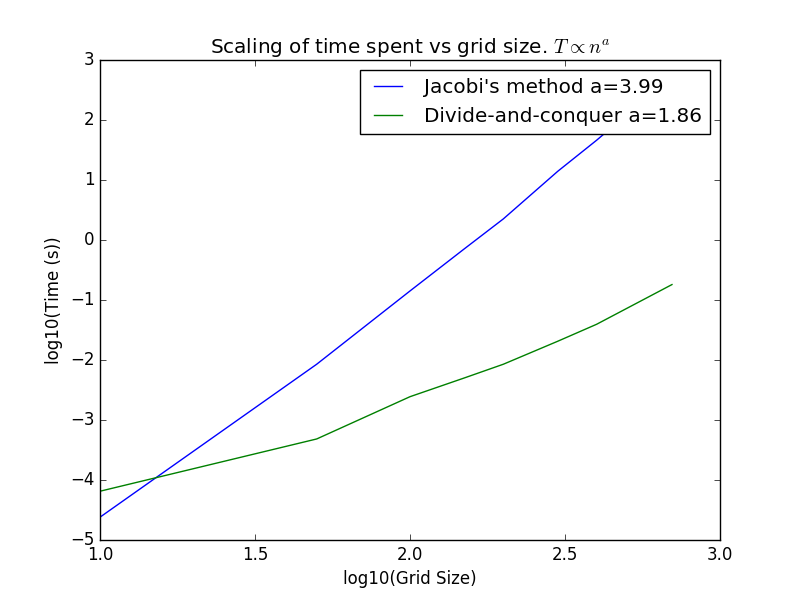
\includegraphics[scale=0.6]{Project2_scaling_time}
	\caption{Scaling of time versus grid size. This data is from a run on a Macbook Pro 13' }
	\label{fig:scaling}
\end{figure}

\section*{Conclusion}
 
		
		
\begin{thebibliography}{3}
			
	\bibitem{M.Hjort-Jensen_CompFys}
	Morten Hjort-Jensen
	\emph{ Computational Physics Lecture Notes Fall 2015}
	Department of Physics, University of Oslo
	2015
	\url{https://github.com/CompPhysics/ComputationalPhysics/blob/master/doc/Lectures/lectures2015.pdf}
			
			
			
			
			
\end{thebibliography}
		
		
		
		
		
		
		
		
		
%__________________________________________________________________________
\end{document}